\documentclass[prc,12pt,nofootinbib,letterpaper]{revtex4}
%\documentclass[12pt]{article}

\usepackage{graphicx}
\usepackage[space]{grffile}
\usepackage[final]{pdfpages}
\usepackage{color}
\usepackage{multirow}
\usepackage{epsfig}
\usepackage{wrapfig}
\usepackage{rotating}
\usepackage{amsmath}
\usepackage{footmisc}
\usepackage{titlesec}
\usepackage{array}
\usepackage{float}
\usepackage{hyperref}
\usepackage[all]{hypcap}
\usepackage{setspace} 

\newcommand{\justifyheading}{\raggedright}
\titleformat{\section}
  {\normalfont\Large\bfseries\justifyheading}{\thesection}{1em}{}
\titleformat{\subsection}
  {\normalfont\large\justifyheading}{\thesubsection}{1em}{}
\titleformat{\subsubsection}
  {\normalfont\justifyheading}{\thesubsubsection}{1em}{}
\renewcommand*{\thesection}{\arabic{section}}
\renewcommand*{\thesubsection}{\thesection.\arabic{subsection}}
\renewcommand*{\thesubsubsection}{\thesubsection.\arabic{subsubsection}}

\begin{document}

\title{\bf{\Large Silicon Microstrip Sensors for SiD:} \\  R\&D Review and Future Plans}

\author{M. Breidenbach, C. Kenney, T. Nelson, A. Tomada \\ \textit{SLAC National Accelerator Laboratory}}

%\input{author_list}

\date{\today}

\begin{abstract}
\vspace{0.5cm}

\begin{centerline}
{\bf {EXECUTIVE SUMMARY}}
\end{centerline}
\begin{singlespace}

The SiD detector concept for a future $e^+e^-$ collider (e.g ILC, CLIC) includes a large volume silicon microstrip tracker consisting of more than 10000 individual sensors.  These sensors employ a second metal layer to provide connectivity to a surface mounted readout ASIC, KPiX, via bump bonds and a polyimide cable via wire bonds. A set of prototype sensors was manufactured by Hamamatsu in 2008. After exhaustive attempts to form connections to the sensors utilizing a number of different technologies, we find that we are unable to make reliable and robust connections to either the ASIC or the cable that would allow the sensors to be tested and utilized for R\&D and prototyping as intended for the project. While the nature of the problem is clear, the underlying mechanism and required solutions are not well understood.  However, given the history of success in fabricating similar sensors that would meet our requirements, we are confident that solutions exist and that another batch of sensors can be made with different processing that will allow us to continue the development and prototyping of the SiD detector.

\end{singlespace}
\end{abstract}

\maketitle

\section{Introduction}

A key element of the SiD detector concept for the ILC is a large silicon tracker, consisting of over 10000 large silicon microstrip sensors. These sensors are quite conventional in most respects; single-sided, p$^+$-in-n bulk, AC-coupled, polysilicon-biased sensors fabricated on 320 $\mu$m thick,  6-inch wafers of $<$100$>$ silicon.  However, these sensors utilize a novel readout scheme to eliminate the material and complexity of a hybrid circuit board to house the front-end readout electronics.  Instead, the readout ASICs, KPiX, are bump bonded directly to the surface of the sensor, where a second metal layer is used to route the signals from the AC-coupled sense strips to the bump bond pads for KPiX.  Additionally, the second metal layer includes traces for power and digital control of KPiX that terminate at wirebond pads for wirebonding to a polyimide flex cable glued to the face of the sensor. This cable connects KPiX to the external DAQ and power supply, as well as providing bias to the sensor.  As shown in Figure~\ref{fig:module}, the design calls for each sensor to be read out by a pair of 1024-channel bump-bonded KPiX, which are controlled and read out by a single cable which attaches to the sensor between the two readout chips.
%=======================
\begin{figure}[htbp]
\begin{center}
    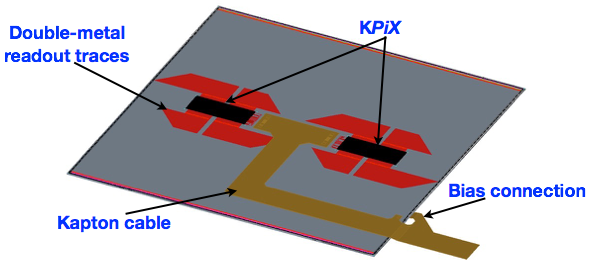
\includegraphics[width=\textwidth]{figures/module}
\caption{The module concept for the SiD outer tracker.  Each sensor is read out by a pair of KPiX readout ASICs via a polyimide flex cable, which also provides bias to the sensor.}
\label{fig:module}
\end{center}
\end{figure}
%=======================
In early 2008, after extensive development of the sensor design and specifications in cooperation with Fermilab and Hamamatsu, an order was placed for 20 sensors for production of prototype sensor modules to allow testing and further development of this concept.  In addition to the 20 full-sized sensors (93.531$\times$93.531 mm$^2$), the mask design included 40 smaller test sensors, each of which included a bump bond pattern allowing the connection of smaller prototype versions of KPiX having between 64 and 256 channels.  These test sensors were intended to allow all of the various connection and crosstalk issues to be tested prior to prototyping with the full-sized sensors.  The specifications and drawings for these sensors are shown in Appendix~\ref{sec:specs_drawings}.


\section{Results with Test Sensors}

On March 29, 2008, Hamamatsu delivered these sensors to Fermilab and the smaller test sensors were immediately sent to SLAC for initial testing and assembly.  Because the bump-bonding process for KPiX was still under development, the first test called for gluing a 64-channel KPiX prototype upside-down (with bump bond pads facing upwards) to allow wirebonding to the test sensor.  The primary purpose of this test was to assess crosstalk from KPiX clock traces that are routed on the second metal layer to the underlying sense traces. The wirebonding layout for this test is shown in Figure~\ref{fig:wirebond-test}. 
%=======================
\begin{figure}[htb]
\begin{center}
    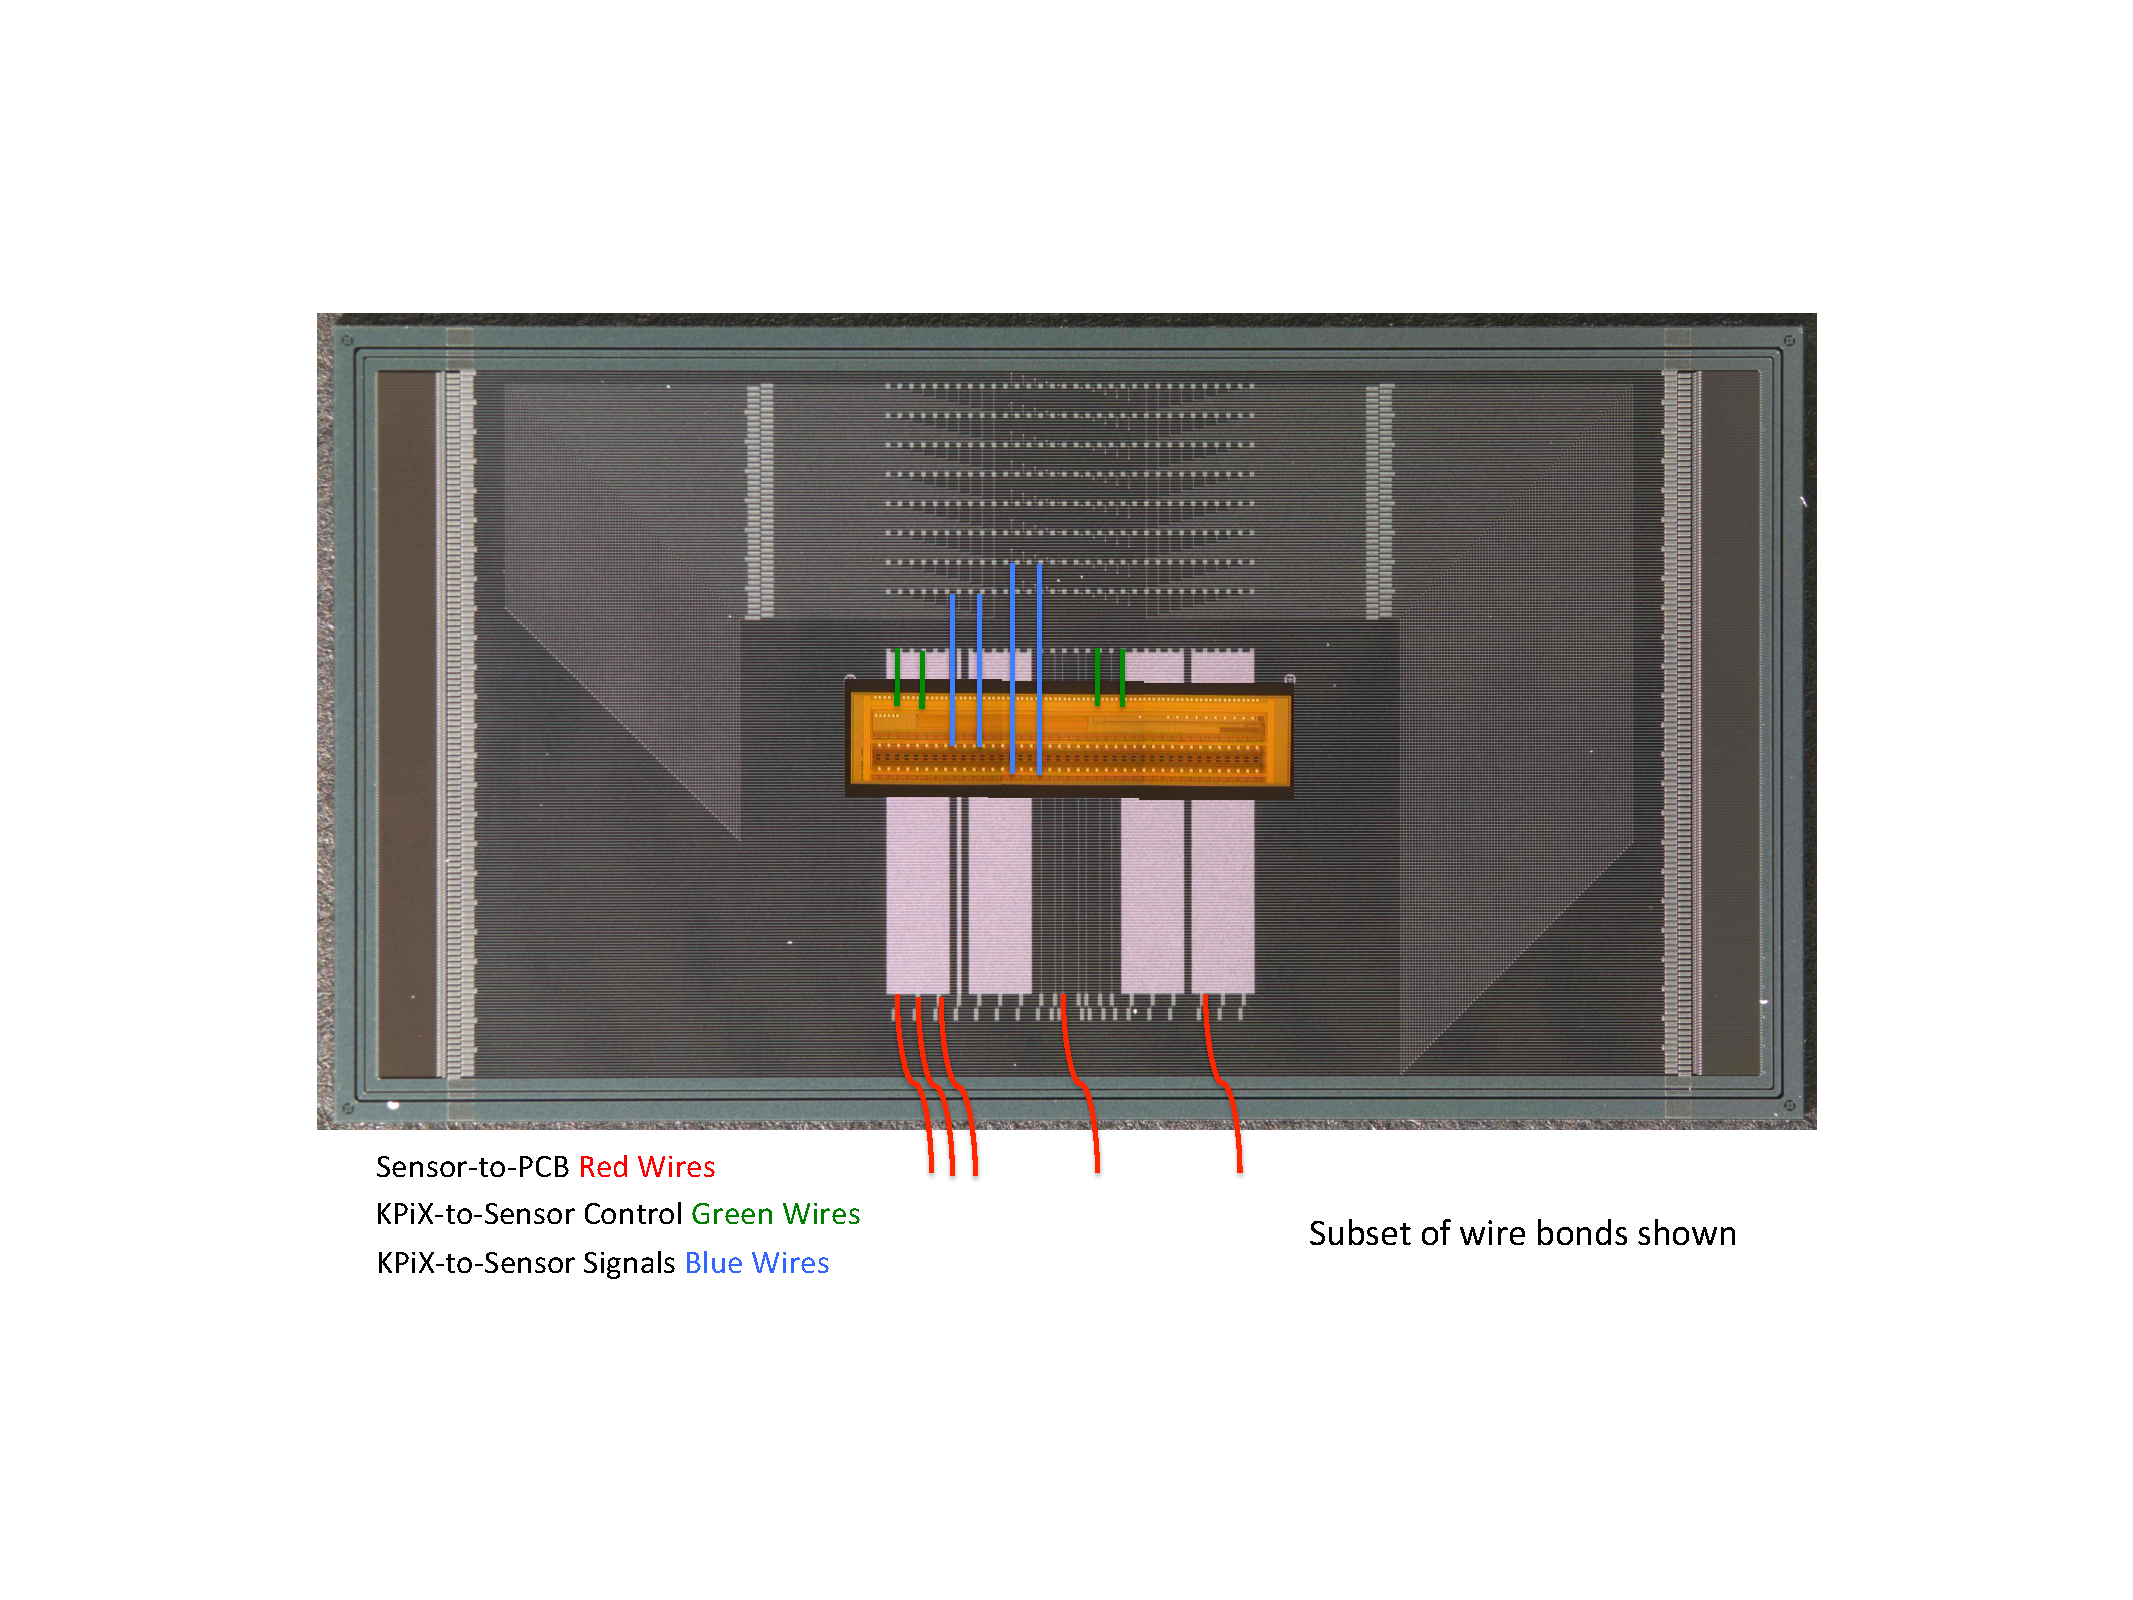
\includegraphics[width=6in]{figures/wirebond-test}
\caption{The layout for initial testing with a 64-channel KPiX readout ASIC and double-metal test sensor.  The KPiX is glued to the face of the sensor with bump bond pads facing up to allow wirebonding of KPiX to both the power/control traces (second metal) and the readout traces (first metal) of the sensor.  For this test, the other end of the power/control traces were bonded to an underlying PCB instead of a polyimide flex cable.}
\label{fig:wirebond-test}
\end{center}
\end{figure}
%=======================
This wirebonding was performed by Amtech Microelectronics Inc., the packaging and SMT vendor used by SLAC for all contract assembly and wirebonding.  Although the wirebonds on this prototype appeared successful, testing revealed that the wirebonds on the sensor had shorted the second metal layer to the first-metal readout traces. A second attempt was made with the same vendor with the same results.  In order to have more control over the wirebonding process, further prototypes were sent to colleagues at UC Santa Cruz and wirebonded there on their Hesse\&Knipps BJ820 by an experienced technician.  The results of this effort were similar and, in general, the rate of punch-through during bonding appears to be at least 10\%. Table~\ref{tab:shorts} summarizes the measured resistance between the second metal clock trace and the first metal readout traces that lie underneath the bonding pads on one of these prototypes. Figure~\ref{fig:strip-218} shows a closeup image of the wirebond pad that was found to have only 70$\Omega$ resistance to the underlying readout trace.
%===================
\begin{table}[htb]
\begin{center}
\begin{tabular}{lc}   
\hline \hline 
Strip Number & Resistance to Clock Pad \\      
\hline
215 & $>$10M$\Omega$ \\
216 & $>$10M$\Omega$ \\
217 & $>$10M$\Omega$ \\
218 & $<$70$\Omega$ \\
219 & 2M$\Omega$ \\
220 & 2M$\Omega$ \\
221 & 2M$\Omega$ \\
\hline \hline
\end{tabular}
\caption[]{The resistance between the clock trace (second metal) and the underlying readout traces (first metal) after wirebonding.  Strip 218 is underneath the wirebond pad for bonding the clock trace to the PCB.}
\label{tab:shorts} 
\end{center}
\end{table}
%===================
%=======================
\begin{figure}[htb]
\begin{center}
    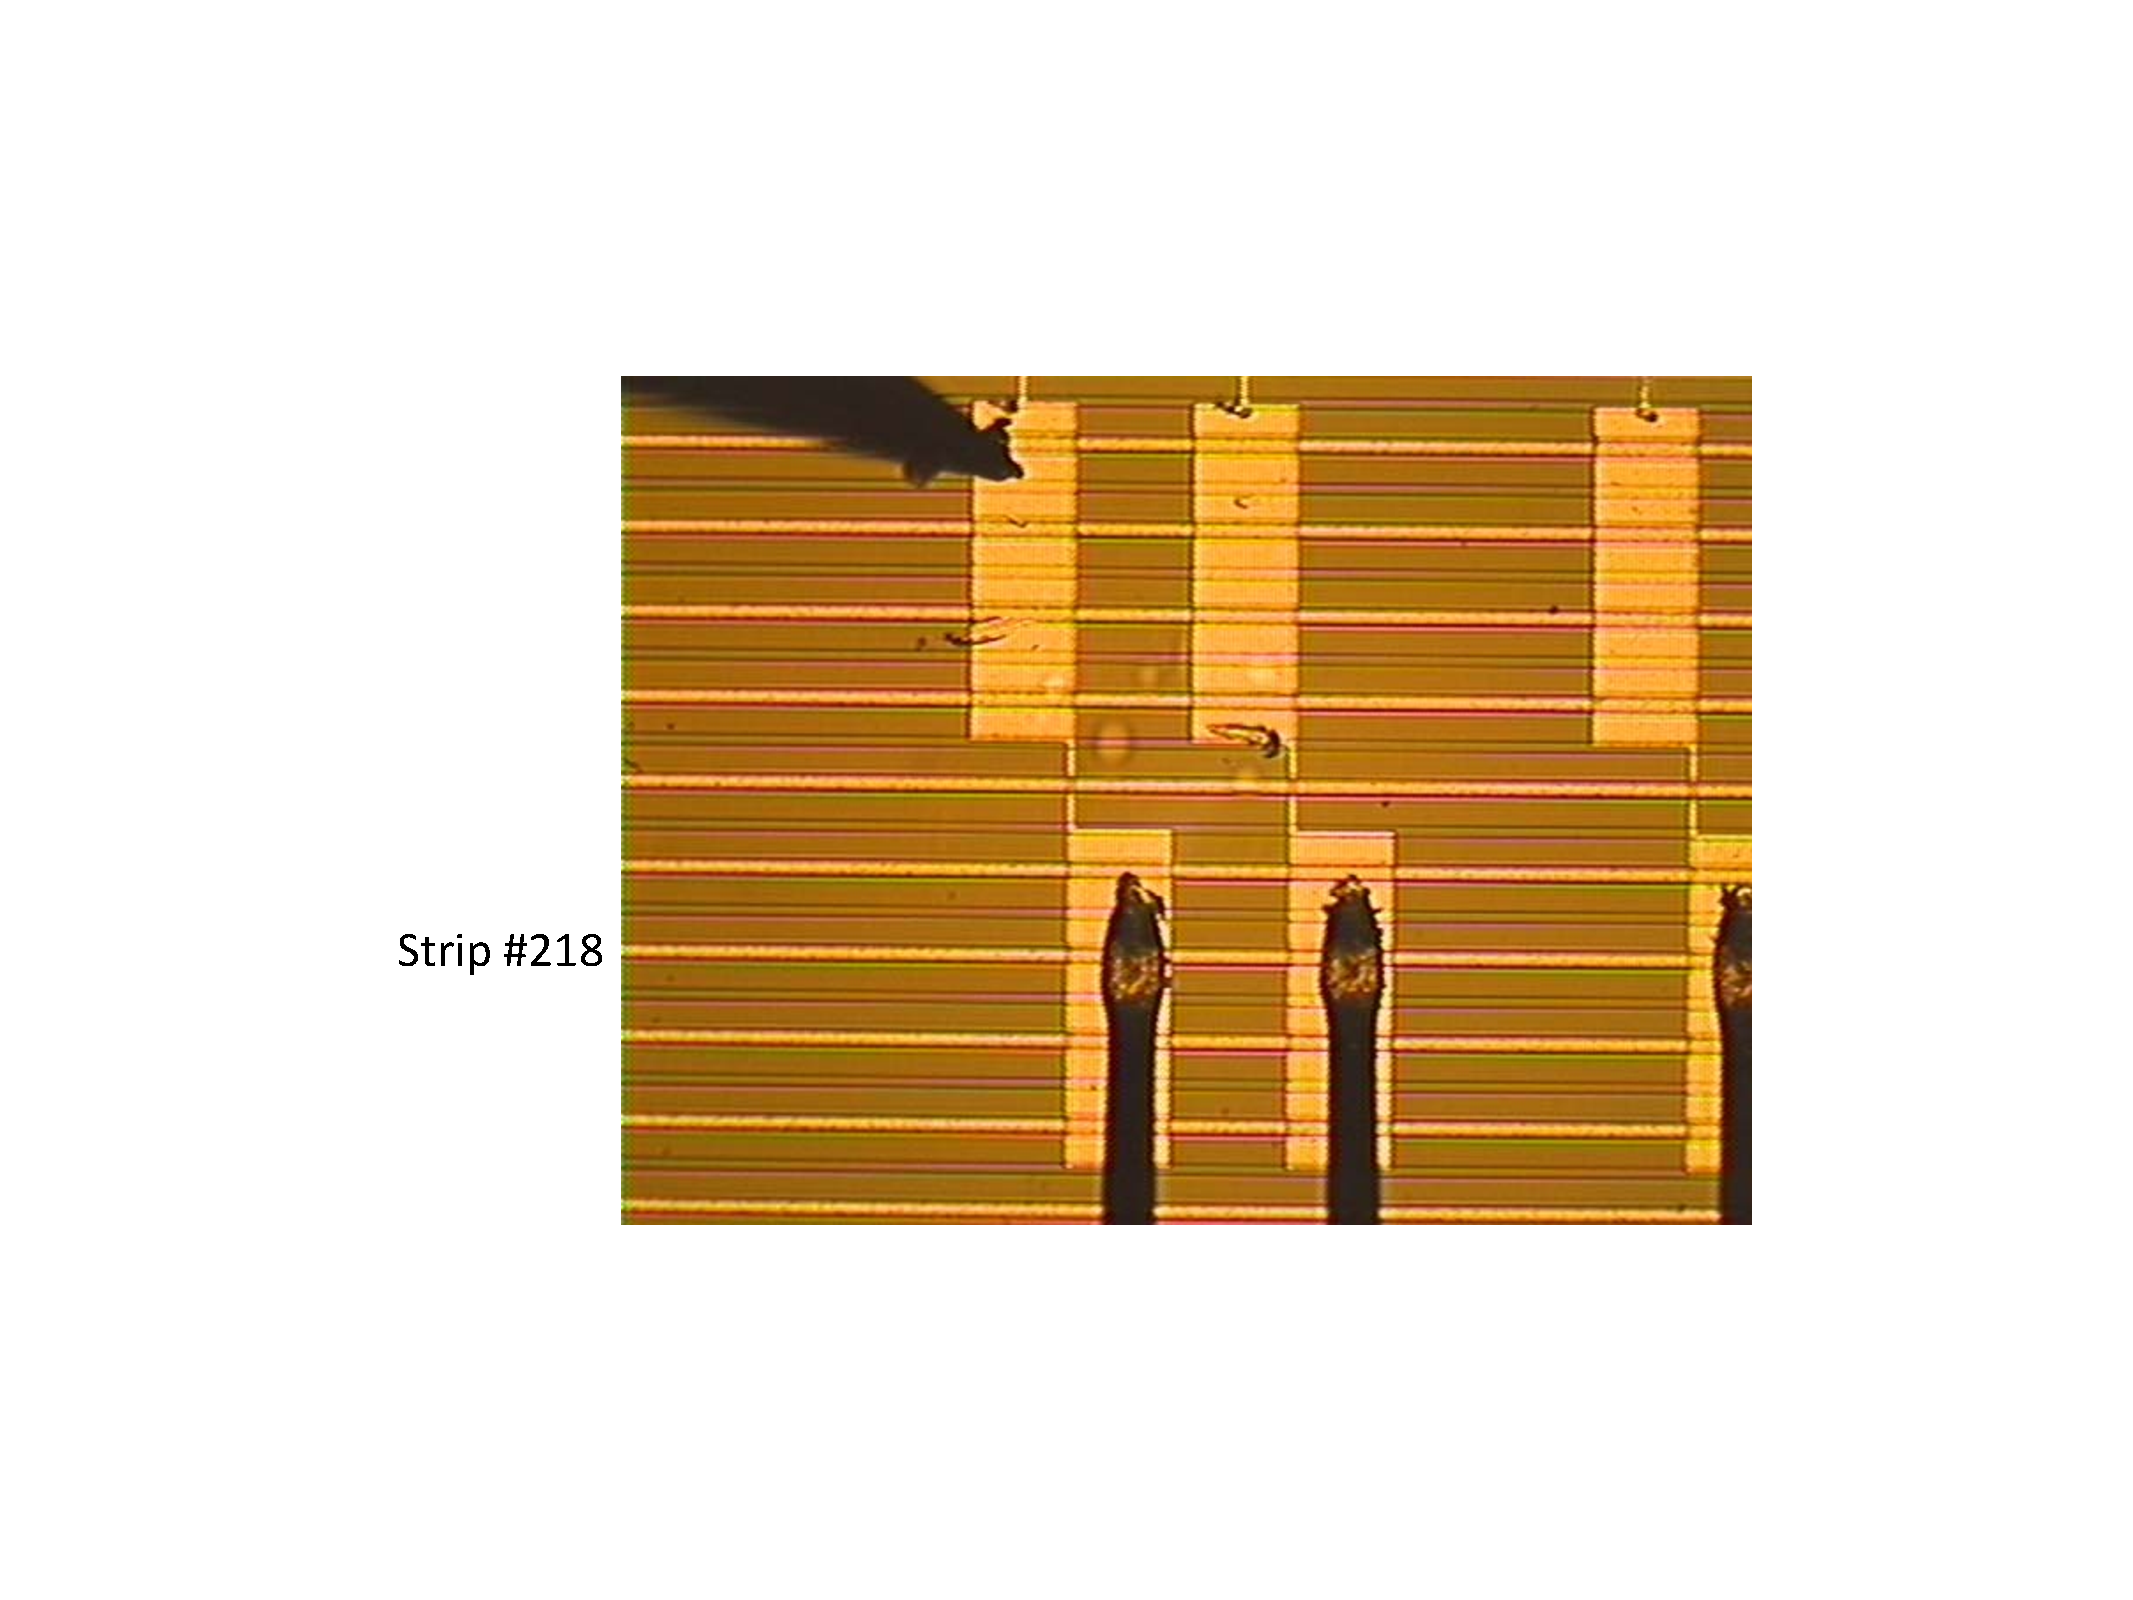
\includegraphics[width=5in]{figures/strip-218}
\caption{The setup for measuring the resistance between the clock trace, shown being probed at the spare wirebonding pad, and the underlying readout traces.  As indicated strip 218 lies underneath the pad where the wirebond was made to the PCB.}
\label{fig:strip-218}
\end{center}
\end{figure}
%=======================
Since then, the same technician using the same machine performed approximately 50000 wirebonds to Hamamatsu sensors fabricated for the D\O\ Run IIb upgrade in producing sensor modules for the HPS experiment without a single failure, resulting in a completed detector with a bad channel rate of less than 0.01\%.  Therefore, it has become clear that the oxide layer between the first and second metal layers on these prototype sensors are, for an unknown reason, simply not robust enough to allow wirebonding.

A number of discussions with Hamamatsu sales and engineering personnel ensued from 2009 to 2011 regarding this problem.  The details of our wirebond testing were shared with Hamamatsu engineers, and SLAC offered to return the sensors to Hamamatsu for evaluation. Although it was clearly the position of SLAC that the sensors were defective and failed a basic requirement, the ability to wirebond without damage, the only offer made by Hamamatsu was to fabricate more sensors with additional passivation between metal layers using the same masks at costs which were similar to the first fabrication order.  Unfortunately, this offer was deemed unacceptable to SLAC, and further discussion of fabricating replacement sensors was dropped.

\section{Results with Full-sized Sensors}

In the ensuing years, progress was made on assembly processes for the similar silicon pad sensor fabricated for the SiD Electromagnetic Calorimeter (ECal) which uses the same readout scheme and KPiX ASIC and was fabricated during the same time period in the same 6-inch process at Hamamatsu.  First, IZM Fraunhofer successfully performed UBM and bump bonding of KPiX chips to the ECal sensors.  Second, the UC Davis group developed a process for solder bonding flex cables; analogous to those for the tracker; to the power, control and bias pads on the sensor: a process which is necessary for the ECal application to maintain a very low stack height.  Therefore, a second version of the polyimide flex cable for the tracker was fabricated for the same solder bonding process to allow connection to the tracker sensor without wirebonding.  

Assembly of the tracker prototype recommenced with sending full-sized tracker sensors to IZM Fraunhofer for the same UBM and bump bonding of KPiX that was performed successfully for the ECal sensors.  However, unlike the ECal sensor, these attempts were unscuccessful.

....

\textbf{DESCRIPTION OF WHAT HAPPENED WITH KPiX BUMP BONDED TO THE TRACKER SENSOR.  (I don't think we should delve into other cable attachment attempts with epoxy, since these only distract from the problem at hand.)}

\section{Status and Future Plans}

After exhaustive attempts to produce and test prototypes of the SiD tracker modules using  sensors procured from Hamamatsu for this purpose, it appears that some defect of design and/or fabrication has resulted in an oxide layer that can withstand neither wirebonding nor bump bonding using industry standard processes.  Meanwhile, the need to complete this R\&D has become more urgent, as the SiD detector concept has matured and the proposals to build a new $e^+e^-$ collider have gained momentum due to the discovery of the Higgs boson at CERN.  Therefore, we now must obtain replacement sensors that will allow us to complete the R\&D as originally intended.  While it is not obvious what change must be made in order to ensure successful fabrication of this design, it is clear that double-metal readout designs similar to the SiD tracker sensor have been successfully fabricated many, many times over the preceding decades by Hamamatsu on 4-inch wafers. Notably, it is our understanding that the standard passivation layer between metal layers in the 4-inch process was 3$~\mu$m, much thicker than the 0.9~$\mu$m oxide used on the 6-inch wafers used for the SiD sensors.    Therefore, it seems reasonable to think that use of a thicker oxide between metal layers might make the sensors more robust to wirebonding.  However, it is less clear what role the thin oxide could play in the failures observed after bump bonding, and given success with the ECal sensors of very similar design (and fabricated during the same period) it is also reasonable to think that some other problem, perhaps in the processing of the tracker sensors, is responsible.

In any case, we would now like to explore the replacement of the SiD tracker sensors, which raises a number of issues.  First, we must insist on some assurance that any replacement sensors do not suffer the same problems. Therefore, some clear acceptance criteria must be set forth by which to judge the robustness of the sensors to wirebonding and/or bump bonding.  Second, in consideration of the failure of the original sensors to meet a fundamental requirement resulting in their total loss after a multi-year effort, we would like production of replacement sensors to take place at a deep discount to the market price.  In particular, we would like to procure 30 sensors in the original design at a cost of no more than \$30000 US. In addition to the standard fabrication, we would like Hamamatsu to deposit the UBM to the bond pads, similar to what was recently done by Hamamatsu on a second batch of sensors for the ECal. Naturally, we would be happy to return the unused portion of the original tracker sensors to Hamamtsu for evaluation in furtherance of our mutual goals of successfully fabricating new sensors.

\appendix

\section{Specifications and Drawings}
\label{sec:specs_drawings}

The specifications for the sensors are shown in Figure~\ref{fig:specs}.  The drawings for the full-sized sensors are shown in Figures~\ref{fig:drawing}, \ref{fig:drawing-readout} and \ref{fig:drawing-ringpads}.   The drawing for the test sensors is shown in Figure~\ref{fig:drawing-testsensor}.
%== Big figures at the end.
%=======================
\begin{figure}[p]
\begin{center}
    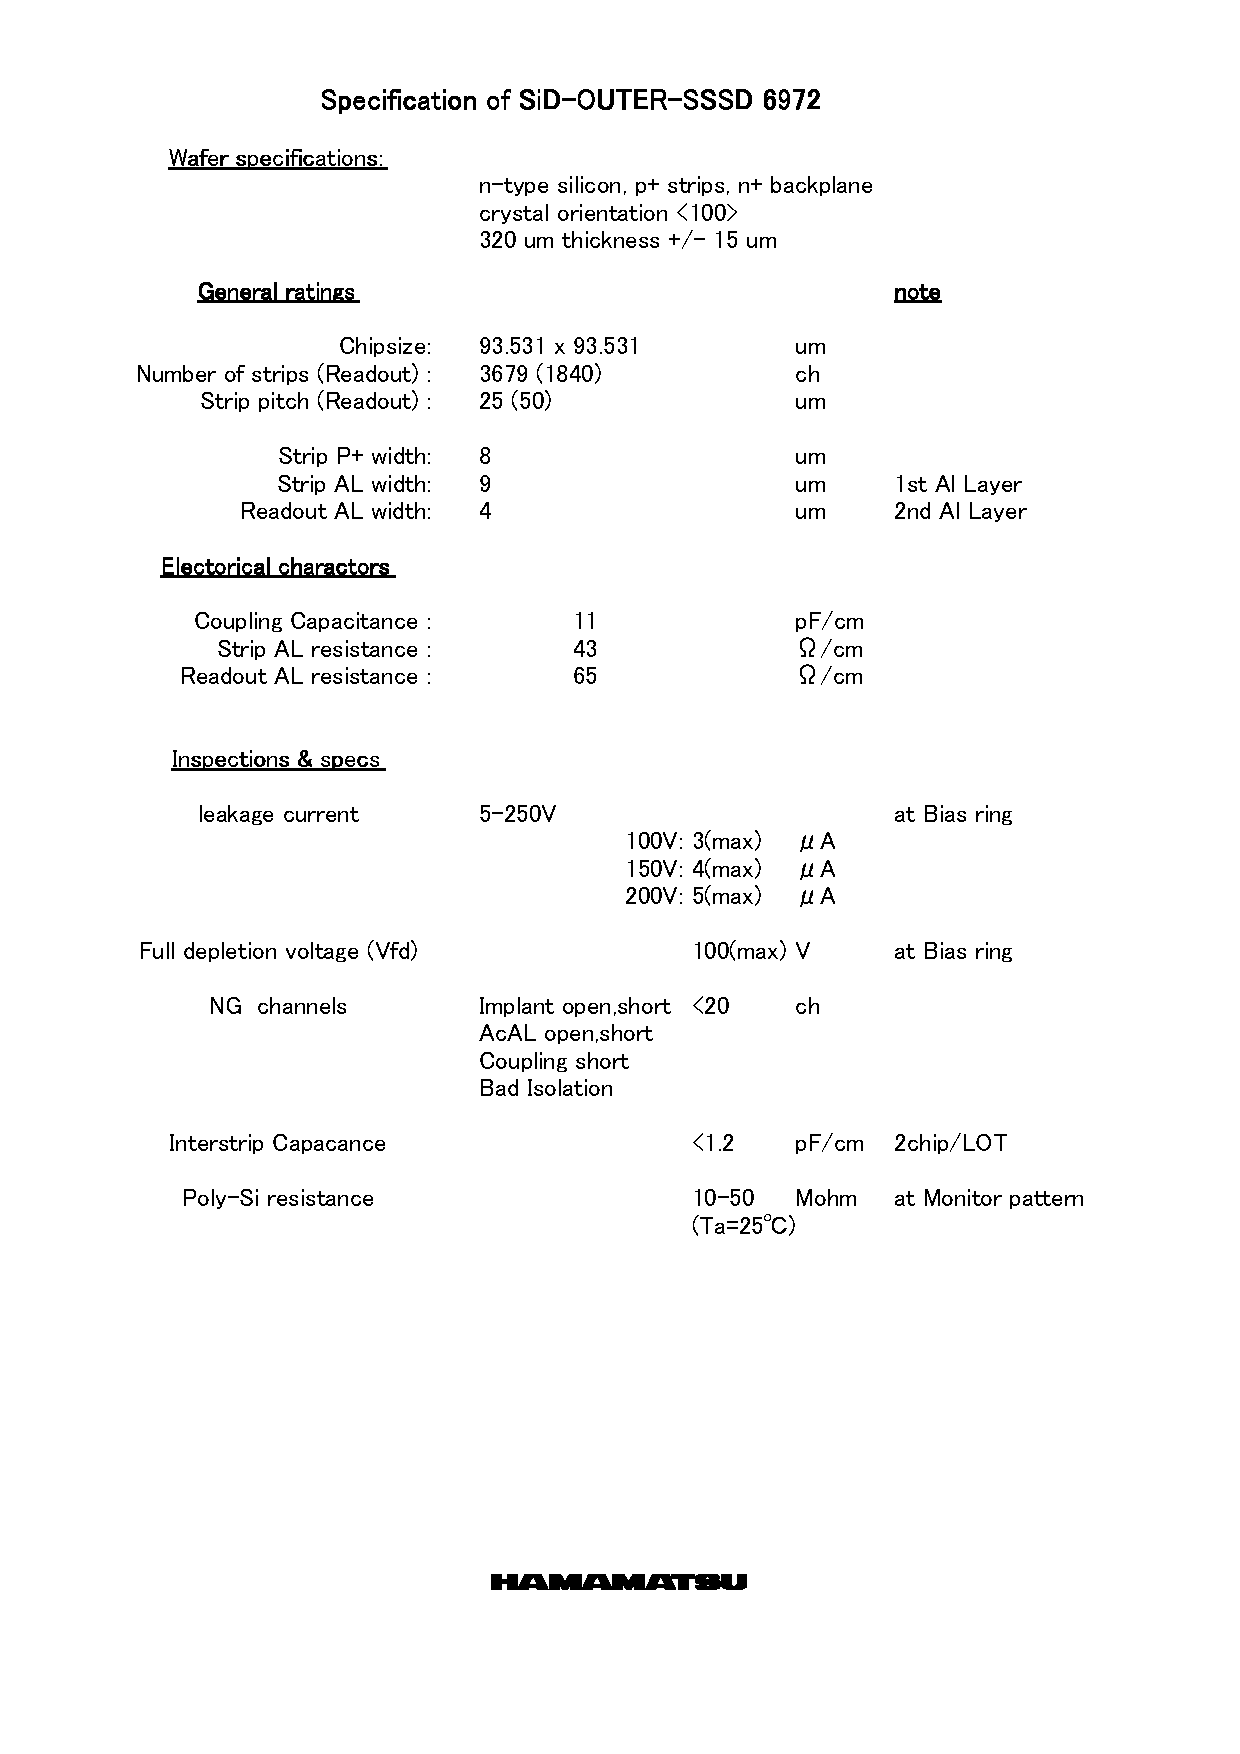
\includegraphics[width=6in]{figures/SiD specsheet 071214}
\caption{The Hamamatsu specifications for the tracker sensor prototypes.}
\label{fig:specs}
\end{center}
\end{figure}
%=======================
\begin{figure}[p]
\begin{center}
    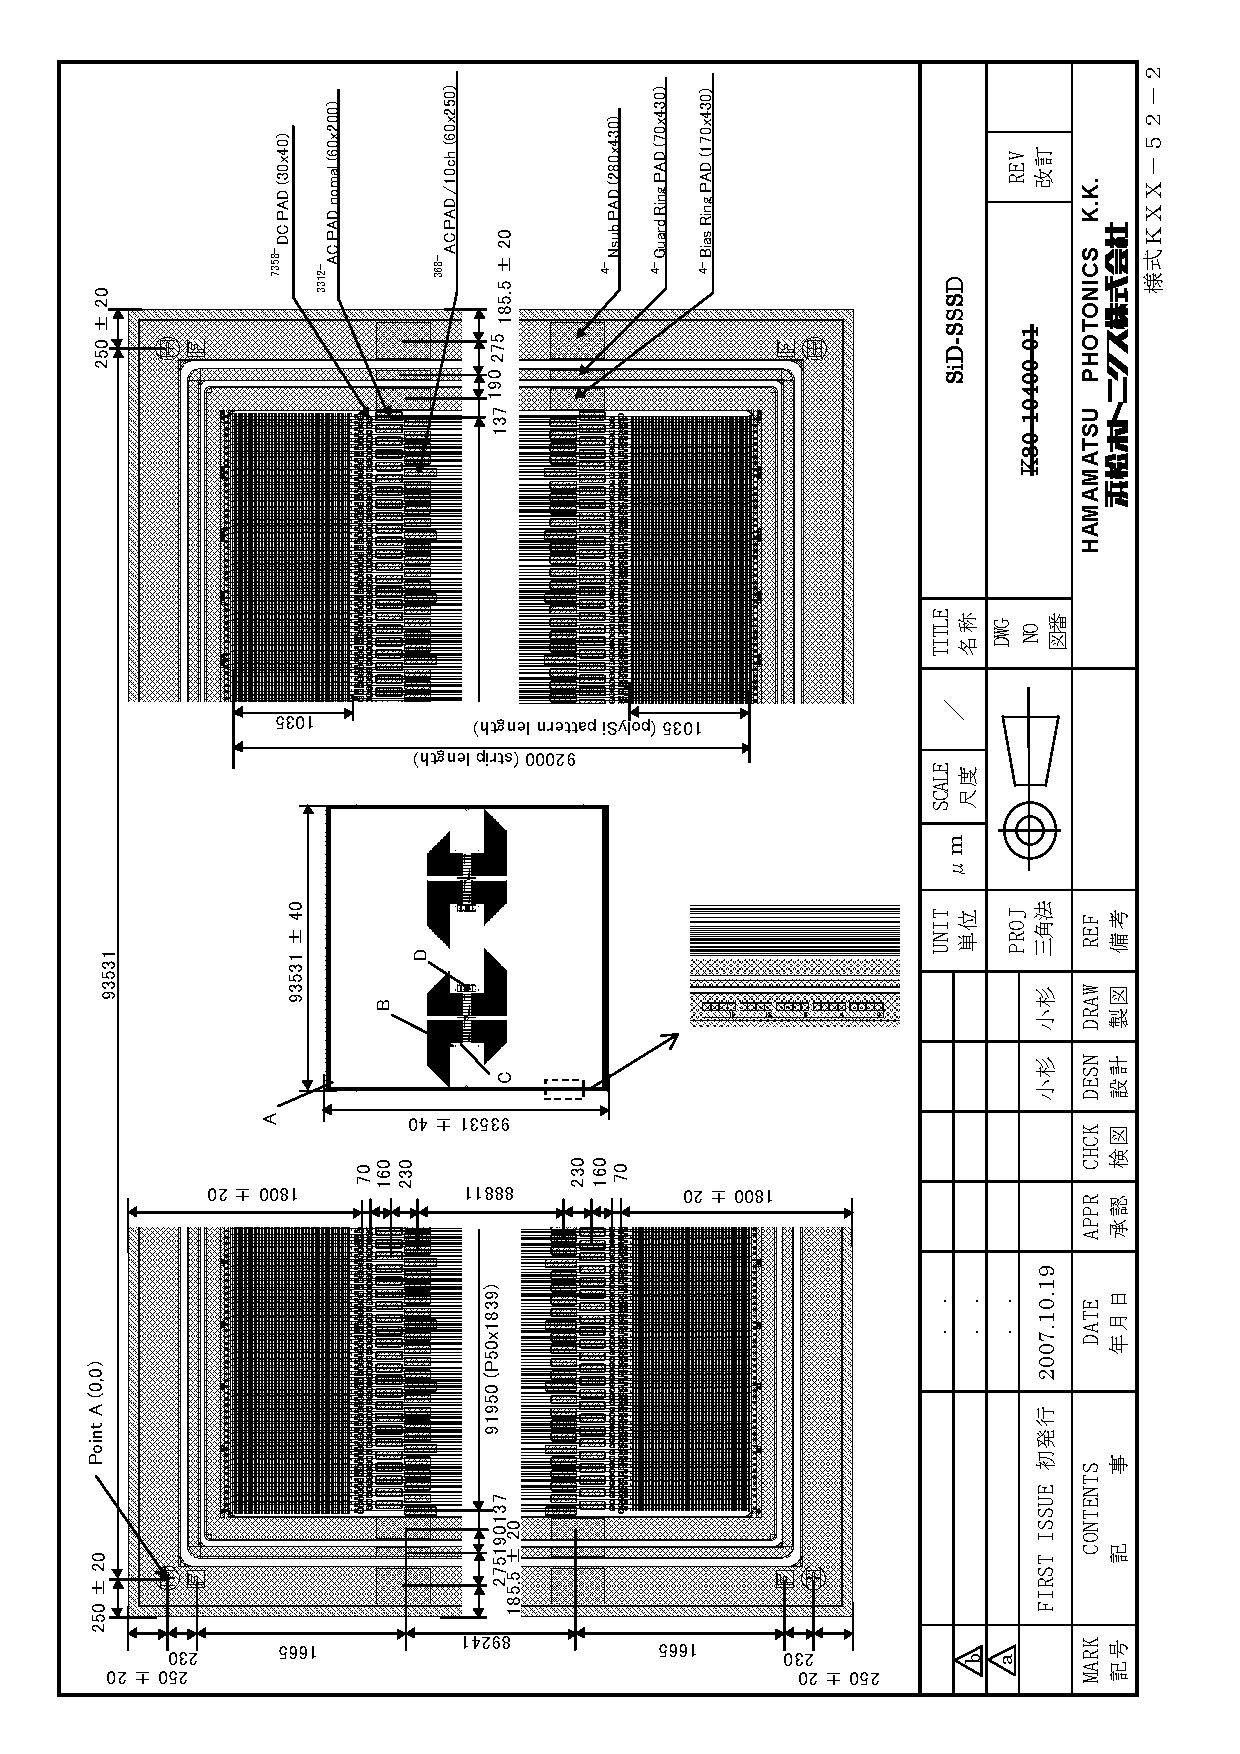
\includegraphics[width=6in]{figures/SiD-SSSD}
\caption{The Hamamatsu overview drawing for the tracker sensor prototypes.}
\label{fig:drawing}
\end{center}
\end{figure}
%=======================
\begin{figure}[p]
\begin{center}
    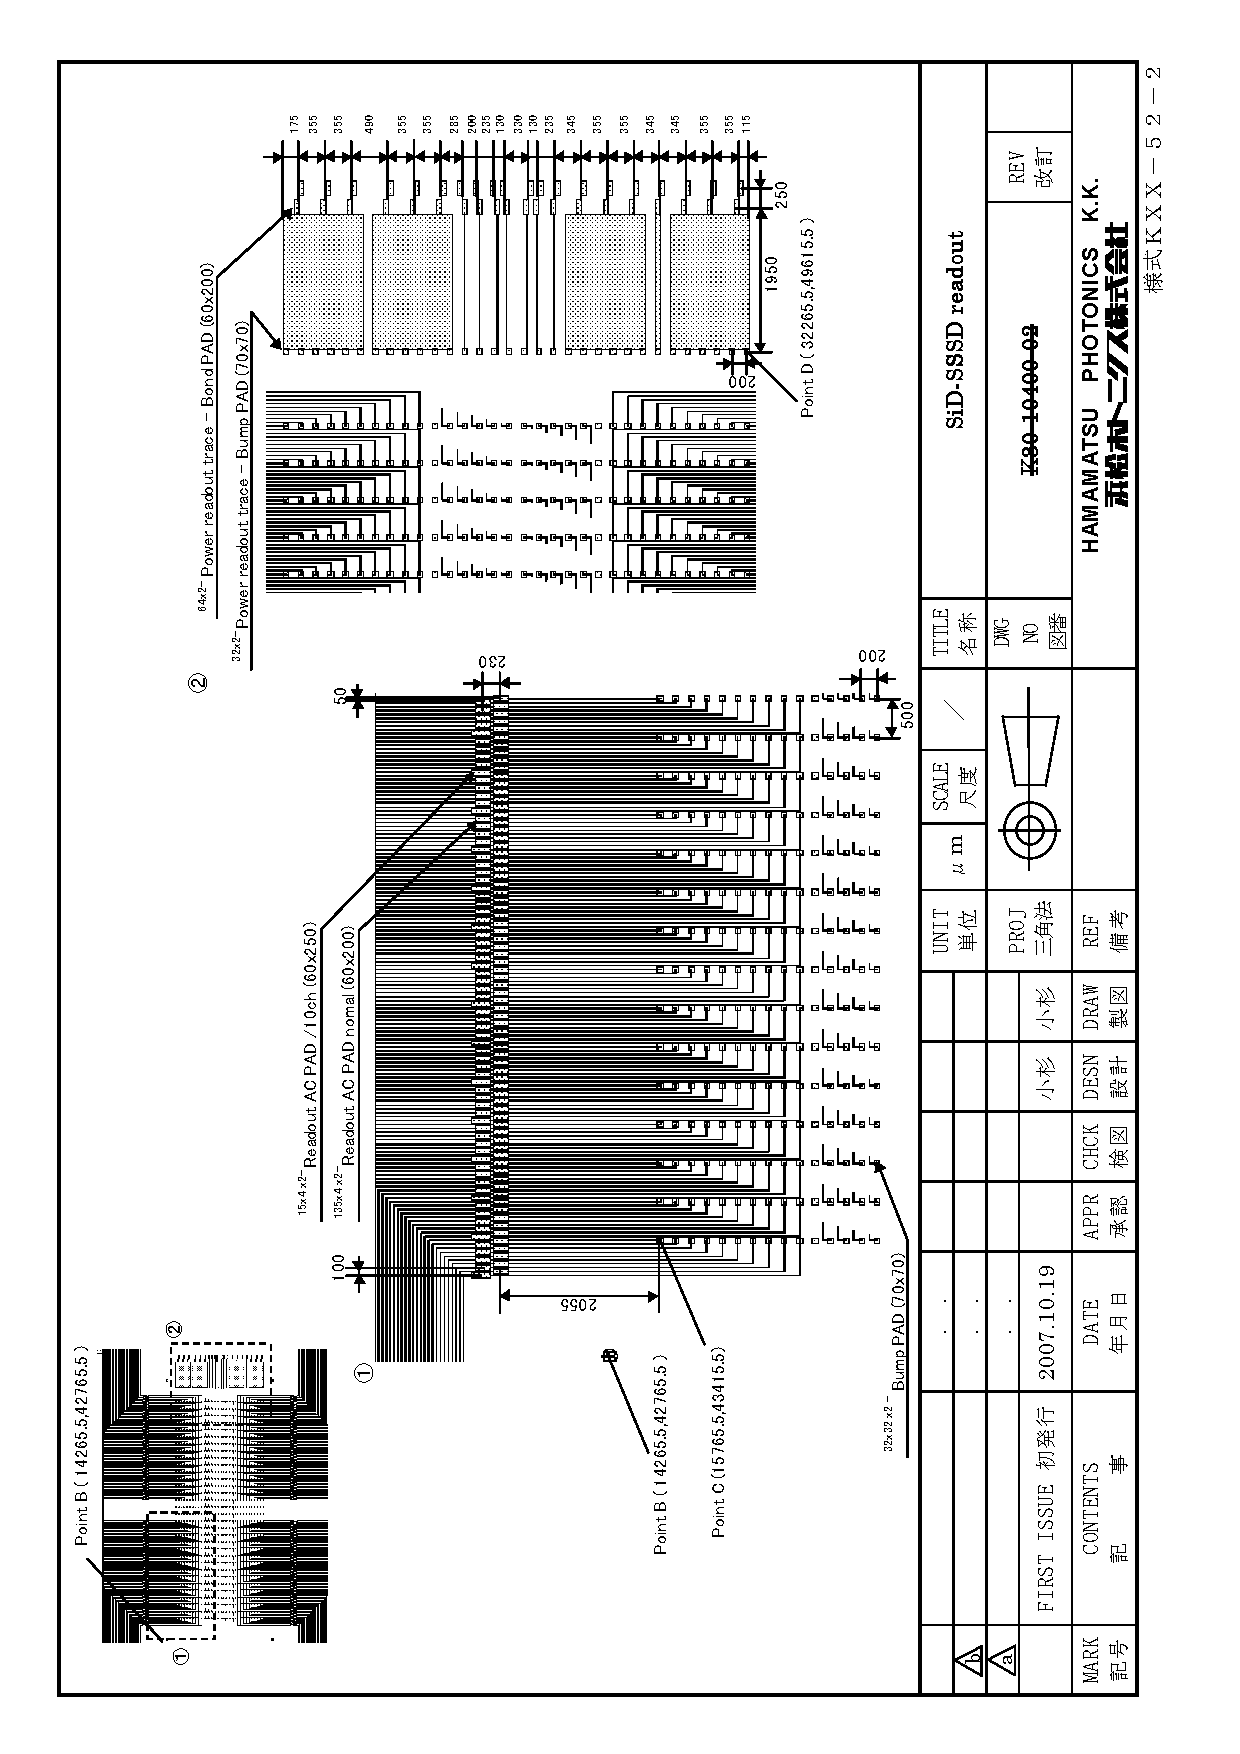
\includegraphics[width=6in]{figures/SiD-SSSD readout}
\caption{The Hamamatsu drawing for the tracker sensor prototypes showing the KPiX and cable bonding region in detail.  The wirebonding pads are along the right edge of the drawing.}
\label{fig:drawing-readout}
\end{center}
\end{figure}
%=======================
\begin{figure}[p]
\begin{center}
    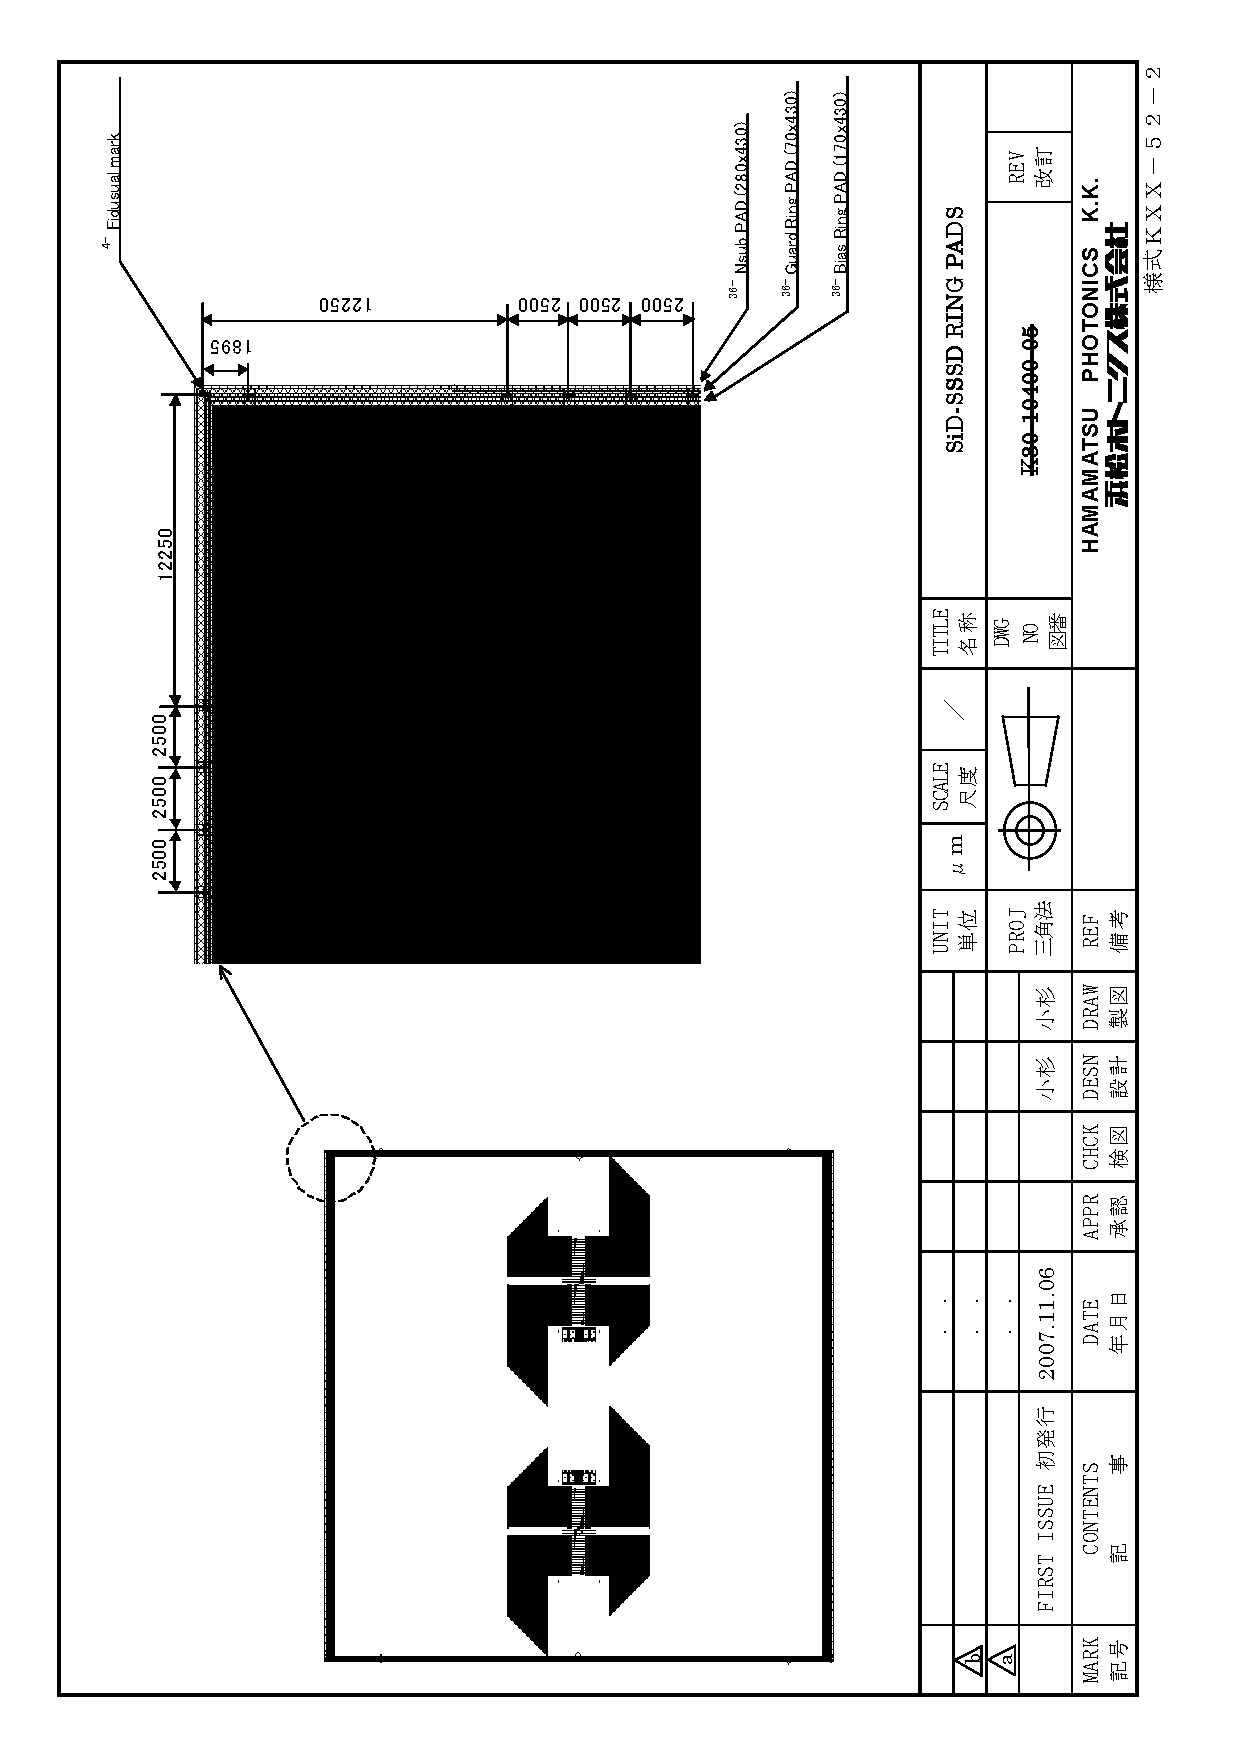
\includegraphics[width=6in]{figures/SiD-SSSD RINGPADS}
\caption{The Hamamatsu drawing for the tracker sensor prototypes showing the bias ring and pads in detail.}
\label{fig:drawing-ringpads}
\end{center}
\end{figure}
%=======================
\begin{figure}[p]
\begin{center}
    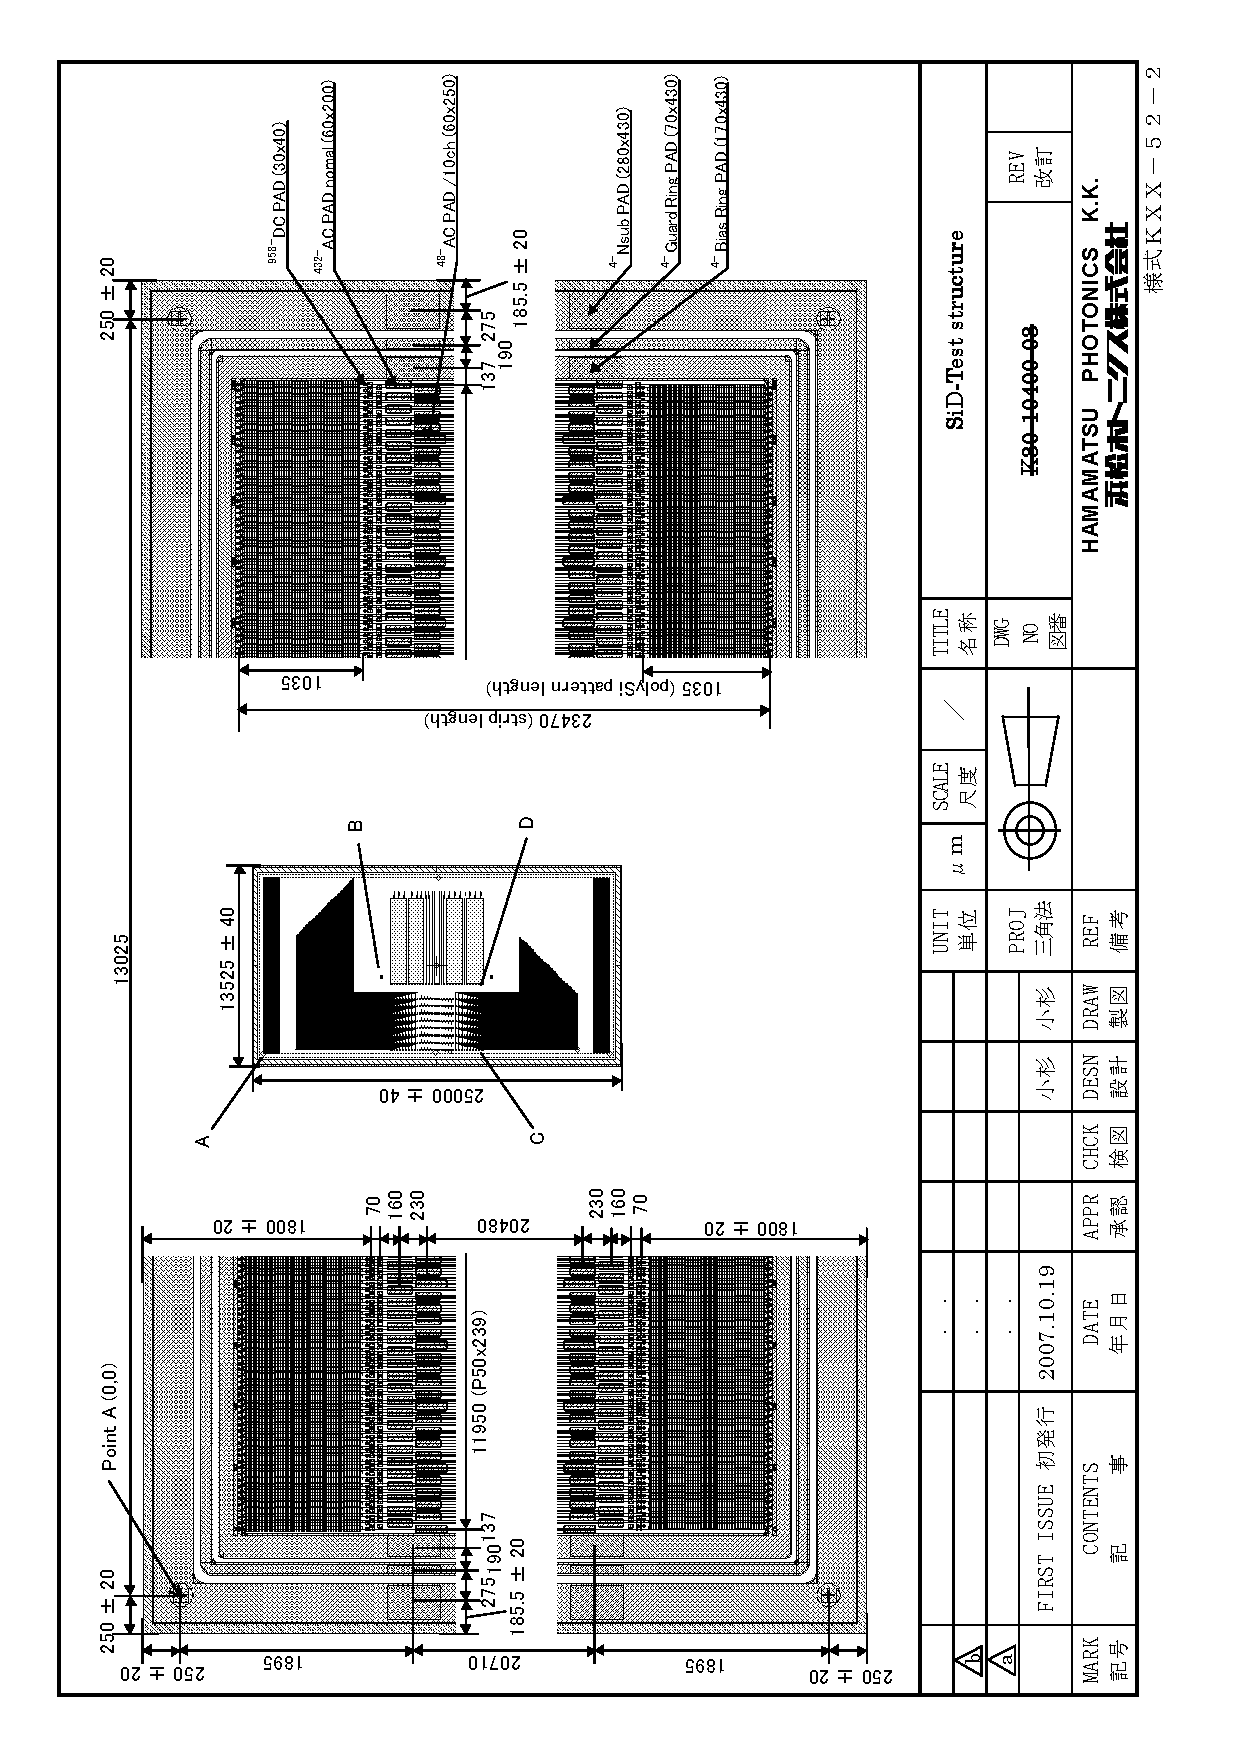
\includegraphics[width=6in]{figures/test structure}
\caption{The Hamamatsu drawing for the test sensors fabricated on the same wafers.}
\label{fig:drawing-testsensor}
\end{center}
\end{figure}
%=======================


\end{document}